%%%%%%%%%%%%%%%%%%%%%%%%%%%%%%%%%%%%%%%%%%%%%%%%%%%%%%%%%%%%%%%%%%%%%%%%%%%%%%%%
\chapter{Разработка}
%%%%%%%%%%%%%%%%%%%%%%%%%%%%%%%%%%%%%%%%%%%%%%%%%%%%%%%%%%%%%%%%%%%%%%%%%%%%%%%%

Креатив.

%%%%%%%%%%%%%%%%%%%
\section{* Подходы к проблеме}
%%%%%%%%%%%%%%%%%%%

***

Основная идея -- спуск по дереву разбора (TXL) от корневого узла к листьям, собирая по пути следования информацию для определения контекста, в котором находятся обрабатываемые/инструментируемые узлы.
Обход «в глубину» (DFS).

%%%%%%%%%
\subsection{Ограничения выбранного метода инструментирования}
%%%%%%%%%

***
Синтаксическое дерево исходного текста программы не содержит циклов по типам узлов -- при спуске от корня к листьям каждый тип узла встречается не более одного раза

%%%%%%%%%%%%%%%%%%%%%%%%%%%%%%%%%%%%%%%%%%%%%%%%%%%%%%%%%%%%%%%%%%%%%%%%%%%%%%%%
\section{Принцип работы системы}
%%%%%%%%%%%%%%%%%%%%%%%%%%%%%%%%%%%%%%%%%%%%%%%%%%%%%%%%%%%%%%%%%%%%%%%%%%%%%%%%

***
Ключевыми идеями системы являются:
\begin{itemize}
  \item Оперирование контекстами инструментирования как некоторыми множествами.
  \item Использование одного прохода по дереву разбора для осуществления требуемых манипуляций (вставки фрагментов программного кода).
\end{itemize}

%%%%%%%%%%%%%%%%%%%
\subsection{Взаимодействие с окружением}
%%%%%%%%%%%%%%%%%%%

***
как будет работать система?

На рис. ~\ref{fig:layout_artefacts} приведена обобщенная схема работы системы инструментирования с позиции манипуляции артефактами, такими как файлы и аргументы командной строки (параметры запуска).

\begin{figure}[!h]
	\centering
	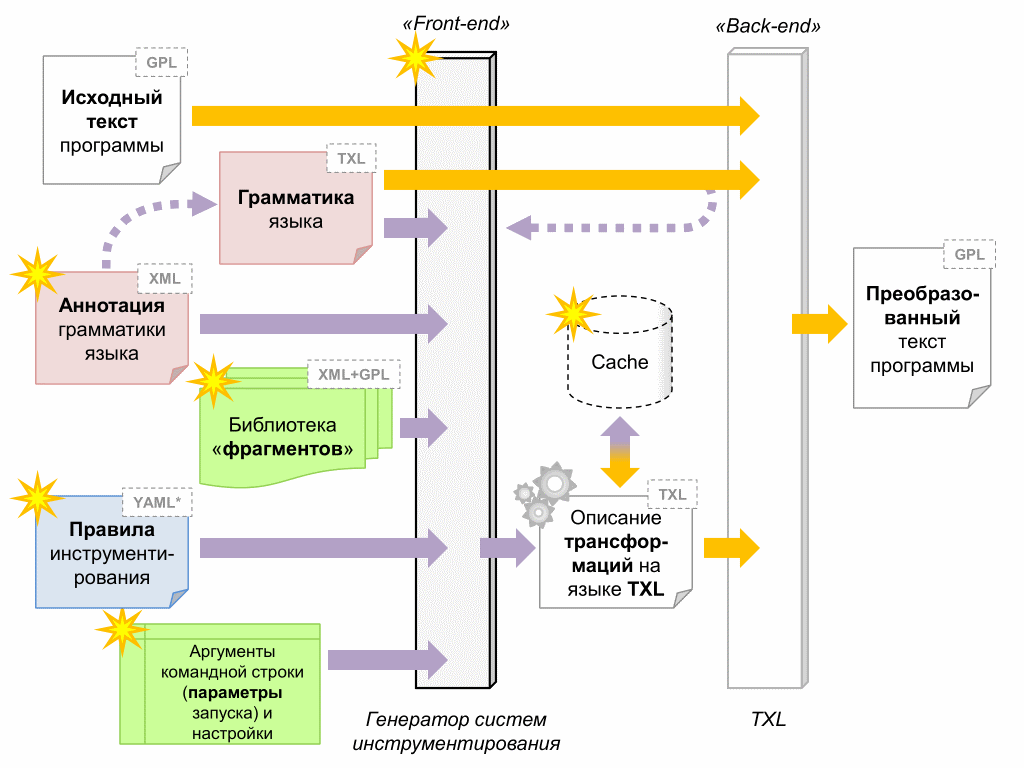
\includegraphics[width=4.2in]{layout_artefacts}
	\caption{Cхема работы системы. Артефакты.}
	\label{fig:layout_artefacts}
\end{figure}

для её работы необходимы:
\begin{itemize}
  \item текст программы, которую нужно инструментировать,
  \item грамматики языка, на котором она написана,
  \item аннотации для этой грамматики,
  \item правила инструментирования, которые пишет пользователь,
  \item фрагменты текста, которые необходимо вставить,
  \item и какие-то дополнительные параметры
\end{itemize}

На рис. ~\ref{fig:layout_users} приведена схема работы системы инструментирования с позиции взаимодействия пользователей и системы как части производственного процесса (создания и отладки программного продукта).

\begin{figure}[!h]
	\centering
	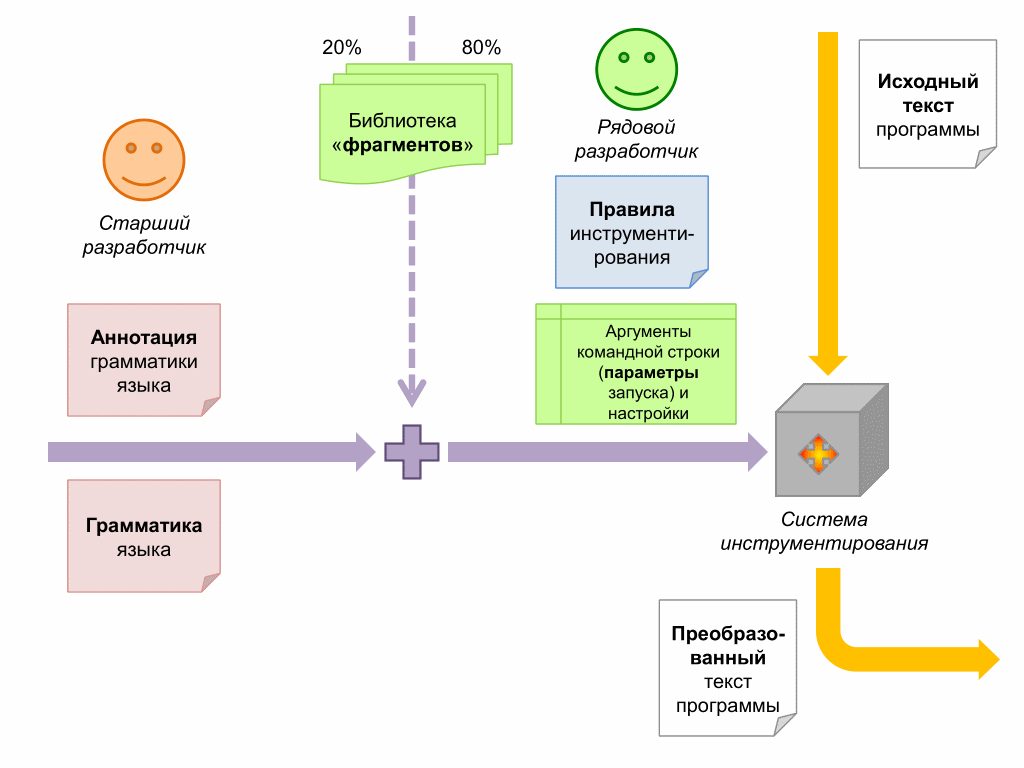
\includegraphics[width=4.2in]{layout_users}
	\caption{Cхема работы системы. Пользователи.}
	\label{fig:layout_users}
\end{figure}

с точки зрения пользователей есть два пльзователя:
\begin{itemize}
  \item более опытный пользователь, в лице старшего разработчика, пишет грамматику и аннотацию к ней, составляет парочку примеров - фрагментов, которые можно вставить.

  \item конечный пользователь, в лице рядового разработчика, пишет правила инструментирования, пишет большую часть текста, который нужно вставить, т.е. библиотеку фрагментов и запускает систему на исходном тексте какой-то программы
\end{itemize}

***

%%%%%%%%%%%%%%%%%%%
\subsection{Правила инструментирования}
%%%%%%%%%%%%%%%%%%%

***
про язык

%%%%%%%%%%%%%%%%%%%
\subsection{Аннотация грамматики языка}
%%%%%%%%%%%%%%%%%%%

***
про XML

* Было бы удобно видеть в одном месте упрощенную схему иерархии типов узлов дерева разбора, в которой отображены только наиболее важные понятия, такие как "класс", "метод", "оператор ветвления", "цикл" и др.

%%%%%%%%%%%%%%%%%%%
\subsection{Фрагменты программного кода}
%%%%%%%%%%%%%%%%%%%

***
про XML

%%%%%%%%%%%%%%%%%%%
\subsection{Выходные артефакты генератора}
%%%%%%%%%%%%%%%%%%%

***
про кэш

%%%%%%%%%%%%%%%%%%%%%%%%%%%%%%%%%%%%%%%%%%%%%%%%%%%%%%%%%%%%%%%%%%%%%%%%%%%%%%%%
\section{Синтез TXL функций}
%%%%%%%%%%%%%%%%%%%%%%%%%%%%%%%%%%%%%%%%%%%%%%%%%%%%%%%%%%%%%%%%%%%%%%%%%%%%%%%%

Основная идея нисходящего подхода заключается в постепенном спуске по дереву разбора, которое генерирует внутри себя утилита TXL, от корневого узла к листьям, сохраняя по пути следования информацию для определения контекста, в котором находятся обрабатываемые узлы и выполняется инструментирование.

Поскольку язык, который использует утилита TXL принадлежит к семейству функциональных языков программирования, это ограничение заставляет передавать собираемую информацию посредством параметров, с которыми вызываются последующие функции в цепочке.

***

%%%%%%%%%%%%%%%%%%%%%%%
\subsection{Общая структура цепочки вызовов}
%%%%%%%%%%%%%%%%%%%%%%%

\begin{enumerate}
  \item C-функции -- функции сбора информации.
  \item F-функции -- функции фильтрации.
  \item R-функций -- функций уточнения контекста.
  \item I-функции -- функции инструментирования.
\end{enumerate}

Кроме этого необходимо существование:
\begin{itemize}
  \item G-функции -- функции получения узлов, содержащих полезные значения (так называемых ''точек интереса''), из промежуточных узлов дерева разбора, имеющих TXL тип, который описывает какую-либо важную синтаксическую конструкцию целевого языка программирования.
  \item H-функции -- функции проверки принадлежности определенному контексту по передаваемым параметрам.
\end{itemize}

%%%%%%%%%%%%%%%%%%%%%%%
\subsection{Функции сбора информации}
%%%%%%%%%%%%%%%%%%%%%%%

***
C-функции -- функции сбора информации.

%%%%%%%%%%%%%%%%%%%%%%%
\subsection{Функция фильтрации}
%%%%%%%%%%%%%%%%%%%%%%%

***
F-функции -- функции фильтрации.

%%%%%%%%%%%%%%%%%%%%%%%
\subsection{Функции уточнения контекста}
%%%%%%%%%%%%%%%%%%%%%%%

После проверки контекста функцией-фильтром, производится вызов первой функции из последовательности R-функций -- функций уточнения контекста.
***

%%%%%%%%%%%%%%%%%%%%%%%
\subsection{Функция инструментирования}
%%%%%%%%%%%%%%%%%%%%%%%

***
I-функции -- функции инструментирования.

%%%%%%%%%%%%%%%%%%%%%%%%%%%%%%%%%%%%%%%%%%%%%%%%%%%%%%%%%%%%%%%%%%%%%%%%%%%%%%%%
\section{Выводы}
%%%%%%%%%%%%%%%%%%%%%%%%%%%%%%%%%%%%%%%%%%%%%%%%%%%%%%%%%%%%%%%%%%%%%%%%%%%%%%%%

Текст.
